% !TeX spellcheck = hu_HU
%----------------------------------------------------------------------------
\chapter{Architektúra}
%----------------------------------------------------------------------------
Az alkalmazás 3 fő részre bontható frontend, backend valamint adatbázis.
E három réteg együttesen felel azért, hogy a felhasználótól a böngészőn keresztül érkező interakciókat kezelje és az állapotot tárolja.
%----------------------------------------------------------------------------

\section{Adatbázis séma}
Az adatbázis migrációját nem kellett manuálisan végrehajtanom a Prisma–nak köszönhetően. 
A Prisma – amellett, hogy kezeli a migrációkat – egy absztrakciós réteget ad az adatbázisunk és az alkalmazásunk közé olyan szinten, hogy teljesen elfedi az adatbázist a fejlesztő elől.

A tervezés során ennek ellenére mégis relációs adatbázist terveztem, majd ezt ültettem át a Prisma által megkövetelt sémába.
Tanulmányaim során ezzel a tervezési metodikával találkoztam és alkalmazása rögzült, rutin szerűvé vált, így először nehéz volt más szemszögből megközelíteni a problémát.

\begin{figure}[!ht]
  \centering
  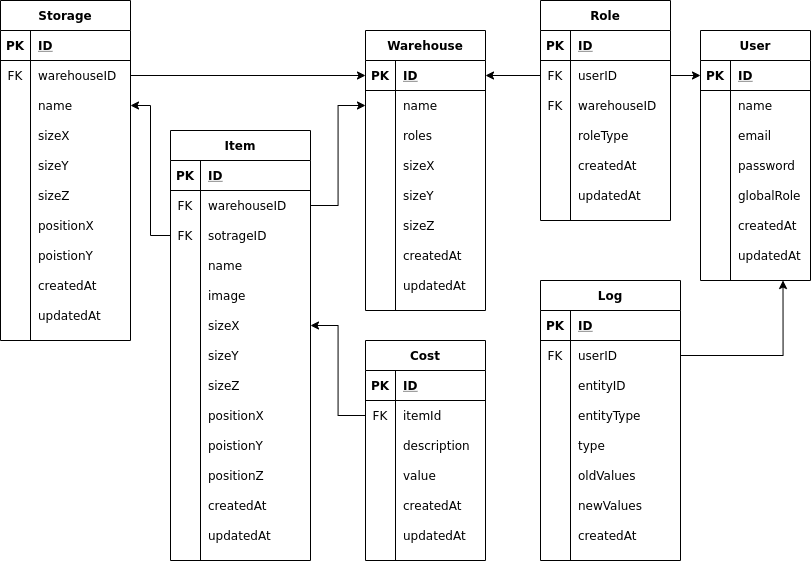
\includegraphics[width=150mm, keepaspectratio]{figures/db.png}
  \caption{Adatbázis séma}
  \label{fig:db}
\end{figure}

Az adatbázis sémát a követelményeket figyelembe véve hoztam létre.
Az ábrán (\refstruc{fig:db}) látható, hogy egy eszköz (Item) tartozhat tárolóhoz (Storage) és raktárhoz (Warehosue) is. 
Erre azért volt szükség, mert a követelmények között szerepelt az ideiglenes tároló fogalma, ami a tárolók közötti eszköz mozgatás megoldását szolgálja.
Ennek megvalósítására új entitás bevezetése felesleges volt. Az opciók között szerepelt még, hogy a tárolók entitásban egy kitüntetett tárolót használunk erre a célra, azonban ez rengeteg elágazást eredményezett volna a kódban.
Így egyszerű tervezési döntés értelmében, ezek a mozgatás során nem tartoznak tárolóhoz csak a raktárhoz, amely ezáltal betölti az ideiglenes tároló szerepét.

A naplózás megvalósításánál törekedtem a generikus megoldás létrehozására.
A napló (Log) tábla csak egy tényleges kapcsolatot tartalmaz a naplóbejegyzés létrejöttét kiváltó felhasználóra mutatva.
A későbbi fejlesztések megkönnyítése érdekében az eszközök és a naplóbejegyzések között nincs tényleges adatbázis kapcsolat.
A kapcsolatot az entitás azonosítója (entityID) és entitás típusa (entityType) határozza meg, így biztosítva, hogy bármilyen entitáshoz készülhessen naplóbejegyzés egységes módon.
%----------------------------------------------------------------------------

\section{Backend felépítése}
Az alkalmazás üzleti logikáját megvalósító rész az architekturális tervezés értelmében egy NodeJS–re épülő rendszer.
Az alkalmazás egyetlen egy végpontot ajánl a kliensek számára.
A kéréseket egy express server fogadja, a feldolgozásának mikéntjéről pedig egy Apollo server gondoskodik, itt történik meg a GraphQL elemzése és ez alapján a megfelelő kódrészlet futtatása.
Az Apollo server lehetőséget nyújt middelware–ek definiálásra, melyek minden kérés kiszolgálása előtt végrehajtódnak.
Erre a lehetőségre épít a GraphQL Shield nevű könyvtár, aminek segítségével minden egyes GraphQL műveletre megadhatunk ahhoz szükséges előfeltételeket egyszerű szabályok segítségével.
Ilyen szabályokkal valósítottam meg a teljes autorizációt és az autentikáció ellenőrzését is.

\begin{figure}[!ht]
  \centering
  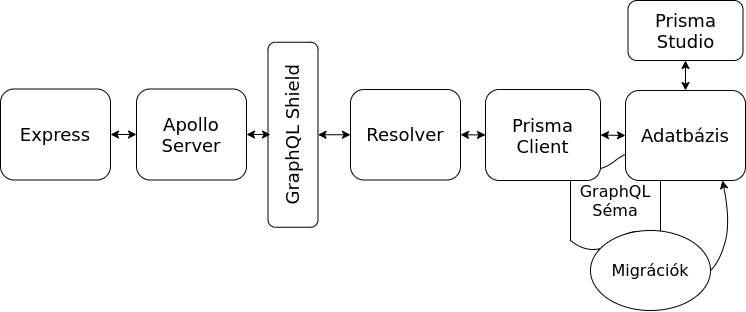
\includegraphics[width=150mm, keepaspectratio]{figures/backend.png}
  \caption{Backend felépítése}
  \label{fig:backend}
\end{figure}

A megfelelő kódrészlet és a middelware–ek futtatása után – a Prisma–án keresztül – az adatbázishoz fordulunk adat lekérés, vagy módosítás miatt.

Az ábrán (\refstruc{fig:backend}) világosan látszik, hogy a Prisma által nyújtott Studio az adatbázishoz csatlakozik, így az általunk írt üzleti logika nem fog érvényesülni.
Fontos, hogy az itt végrehajtott módosítások nem várt működéshez is vezethetnek.

%----------------------------------------------------------------------------

\section{Frontend felépítése}

Ahogy azt a korábbi fejezetekben taglaltam a kliens alkalmazás megvalósításához React–et használtam. Mivel a React önmagában egy nagyon könnyű keretet ad, ezért ezt egy NextJS nevű csomaggal egészítettem ki, amely még kényelmesebbé teszi a használatát.
A backendhez csatlakozást az Apollo Client könyvtárral oldottam meg. 
Az Apollo Client és az Apollo Server együtt egy nagyon jól és könnyen használható rendszert alkotnak.
A Client megkapja a Server–től a GraphQL sémát, így fejlesztés közben kódkiegészítéssel és típus ellenőrzéssel írhatjuk a lekérdezéseinket.
Az Apollo Client a kommunikáció mellett a gyorsírótárazást is kezeli, így biztosítva az alkalmazás lehető leggyorsabb működését.
Ezeken felül lehetőségünk nyílik kódgenerálásra is.
A megírt GraphQL Query és GraphQL Mutation kódokból React hook–okat kapunk, melyekben az állapot– és a típusok kezelése is megvalósított.

\begin{figure}[!ht]
  \centering
  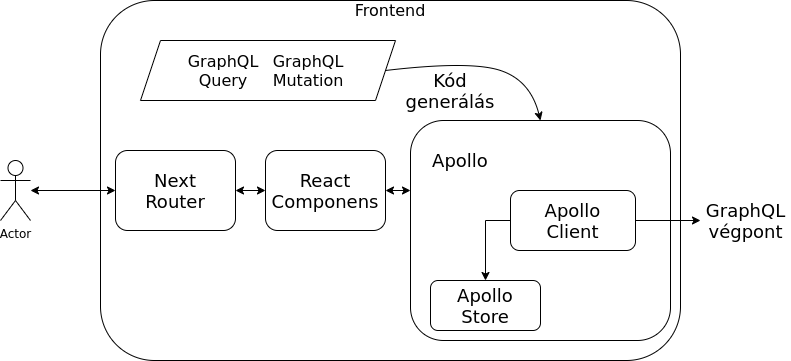
\includegraphics[width=150mm, keepaspectratio]{figures/frontend.png}
  \caption{Frontend felépítése}
  \label{fig:frontend}
\end{figure}

A React–ben a komponensek közötti logika megosztását a Context–ek segítségével valósítottam meg.
Ennek használatával nem szükséges minden komponensnek átadni manuálisan a nélkülözhetetlen változókat, hanem elegendő csak egy, vagy szükség esetén több provider–t az alkalmazásunk köré helyezni.
A provider–ek segítségével adatot szolgáltathatunk az összes provider–en belüli komponens számára.
Elegendő csak az alkalmazás belépési pontjában ezeket a tényleges alkalmazás köré helyeznünk, ahogy azt a mellékelt kód is mutatja.

\begin{lstlisting}[style=ES6, caption=Frontendhez használt provider–ek]    
<ApolloProvider client={client}>
  <ChakraProvider>
    <AuthProvider>
      <Layout>
        <Component {...pageProps} />
      </Layout>
    </AuthProvider>
  </ChakraProvider>
</ApolloProvider>
\end{lstlisting}

%----------------------------------------------------------------------------

\section{Architektúra összefoglalása}
Összegezve az architektúrát, a három fő komponense az alkalmazásnak a frontend, a backend és az adatbázis.
A frontend és a backend közötti kommunikáció GraphQL segítségével történik az Apollo Client és az Apollo Server között.
A backend és az adatbázis kommunikációja pedig SQL segítségével, azonban ezt a Prisma teljesen elfedi a fejlesztő elöl.

\begin{figure}[!ht]
  \centering
  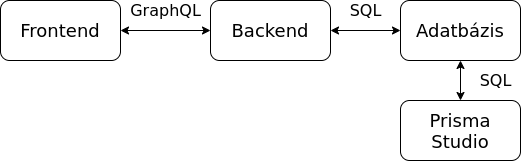
\includegraphics[width=150mm, keepaspectratio]{figures/architecture.png}
  \caption{Teljes alkalmazás felépítése}
  \label{fig:architecture}
\end{figure}